\section{Data}

\textbf{Structure.} Each of the 203,769 nodes is a transaction with a time step
(1--49, about two weeks each) and 165 anonymised features: 93 \emph{local}
features describing the transaction itself (inputs, outputs, fees, amounts, \dots)
and 72 \emph{aggregated} features, statistics of the same quantities over its
one-hop neighbours. Each of the 234,355 directed edges is a flow of bitcoin from
one transaction to another. 77\% of nodes are unlabelled; of the labelled ones,
\EdaIllicitShare{} are illicit.

\textbf{Every time step is a separate graph.} No edge connects two time steps,
and each step forms exactly one connected component (\EdaComponents{} weak
components for 49 steps). This has two consequences we rely on later: graph
statistics computed on the whole graph never mix information across time, and a
graph neural network trained on the full graph cannot pass messages from test
steps to training steps.

\begin{figure}[t]
  \centering
  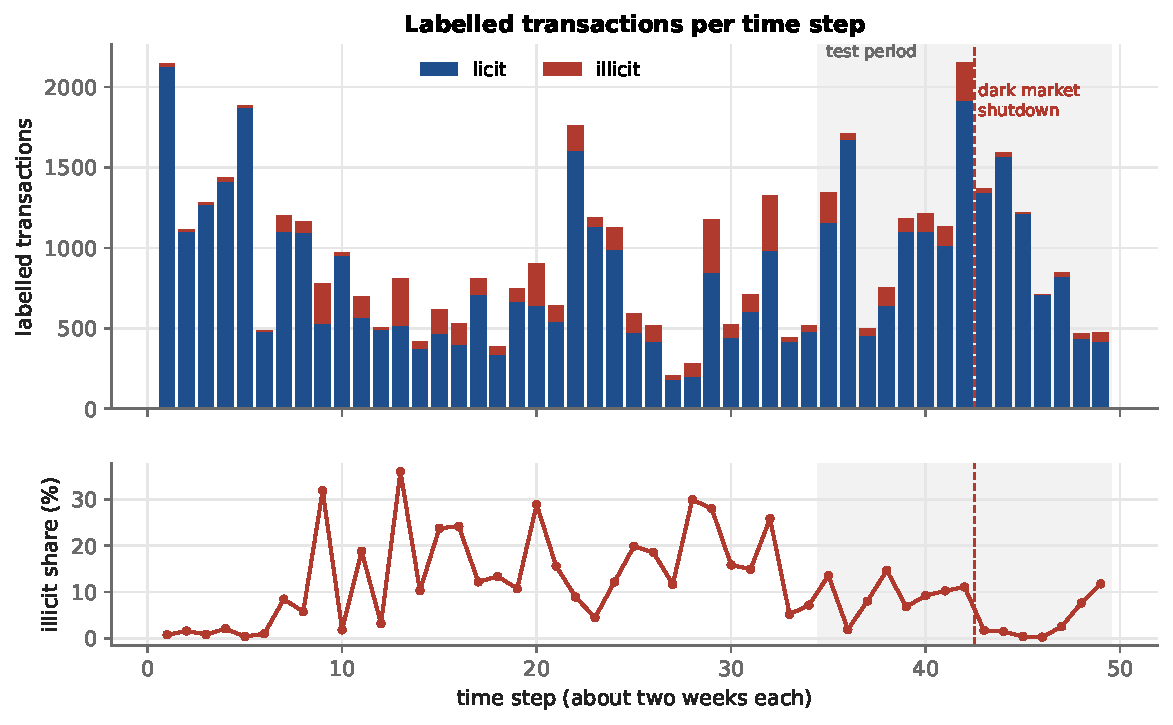
\includegraphics[width=\columnwidth]{../reports/figures/eda_labels_over_time.pdf}
  \caption{Labelled transactions per time step. The illicit share moves between
  0\% and 36\% and falls after the dark market shutdown (dashed line).
  Grey: test period.}
  \label{fig:labels}
\end{figure}

\textbf{Imbalance and its movement over time.} Fig.~\ref{fig:labels} shows that
the illicit share is far from stable: \EdaShareTrain{} in the training steps,
\EdaShareTest{} in the test steps, and almost zero in steps 43--46. Only
\EdaIllicitPost{} illicit transactions occur in steps 43--49, against
\EdaIllicitPre{} in steps 35--42, so the second half of the test period carries
little weight in any pooled metric, and per-step results there are noisy.

\textbf{Redundancy.} \EdaPairsNinetyFive{} feature pairs have $|r|>0.95$; a greedy
filter at that level keeps \EdaFeaturesAfterFilter{} of 165 features
(Fig.~\ref{fig:corr}). Tree ensembles are insensitive to this
redundancy; for the linear model and the MLP we use $L_2$ regularisation instead
of discarding features. In a two-dimensional PCA view (Fig.~\ref{fig:pca}) the
illicit transactions lie inside the licit cloud: no linear projection separates
them, which anticipates the weak result of Logistic Regression.

\begin{figure}[t]
  \centering
  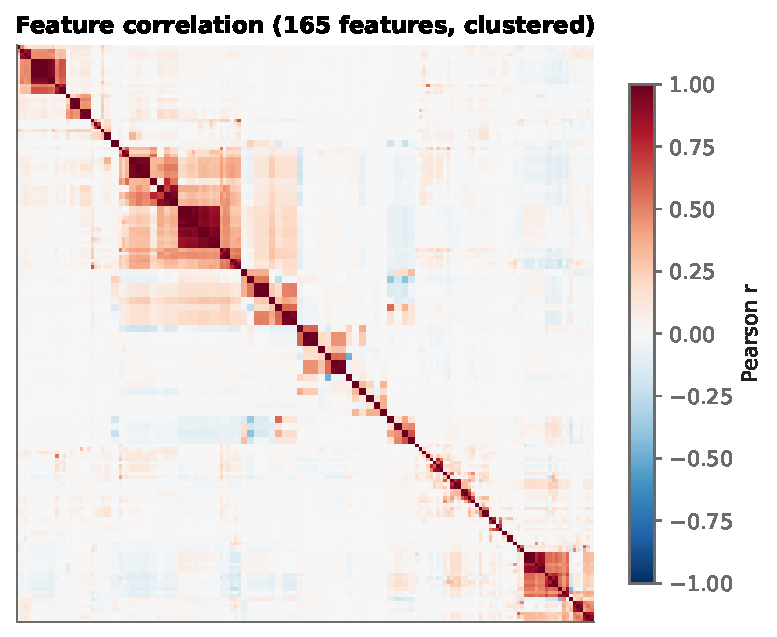
\includegraphics[width=0.78\columnwidth]{../reports/figures/eda_feature_correlation.pdf}
  \caption{Pearson correlation of the 165 features, hierarchically clustered.}
  \label{fig:corr}
\end{figure}

\begin{figure}[t]
  \centering
  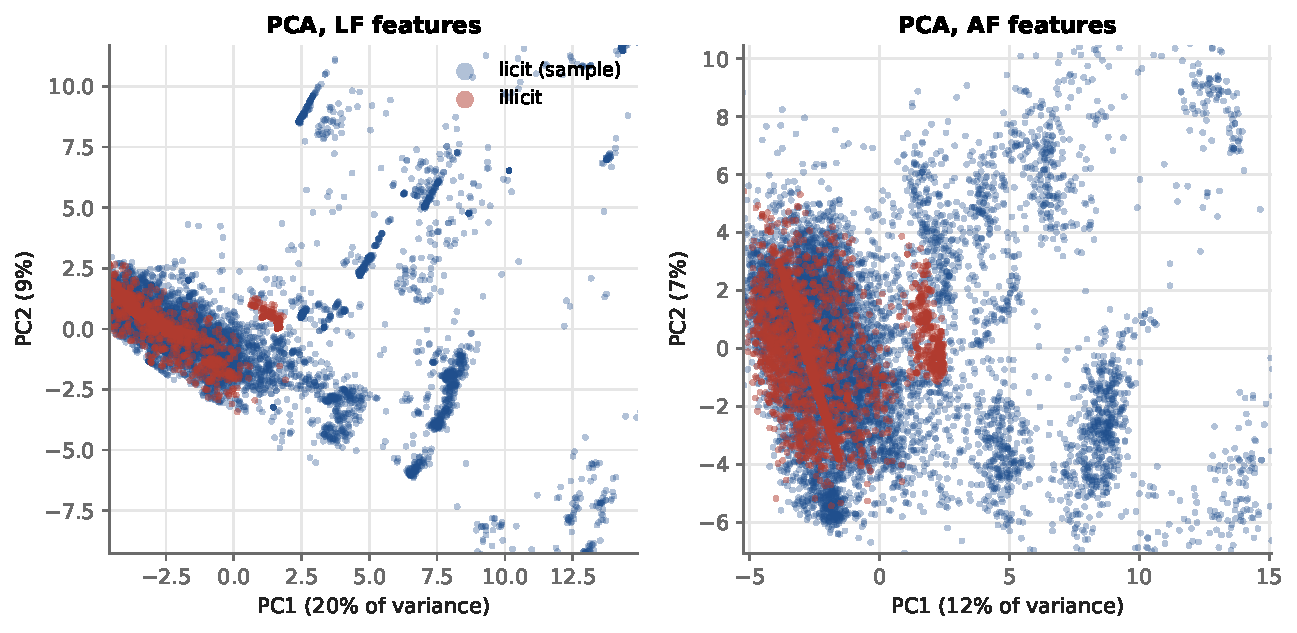
\includegraphics[width=\columnwidth]{../reports/figures/eda_pca.pdf}
  \caption{First two principal components of local (LF) and all (AF) features
  (licit transactions subsampled).}
  \label{fig:pca}
\end{figure}

\textbf{The graph carries label information.} Of the labelled neighbours of an
illicit transaction, \EdaHomIll{} are illicit, against \EdaHomLic{} for a licit
transaction (base rate \EdaHomBase{}). Illicit transactions cluster in the graph.
Their shape also differs (Fig.~\ref{fig:degree}): no illicit transaction has more
than three outputs, while licit ones reach hundreds, yet some illicit
transactions collect up to $\sim$180 inputs. Direction matters, which motivates
the directed GNN of Section~\ref{sec:method}.

\begin{figure}[t]
  \centering
  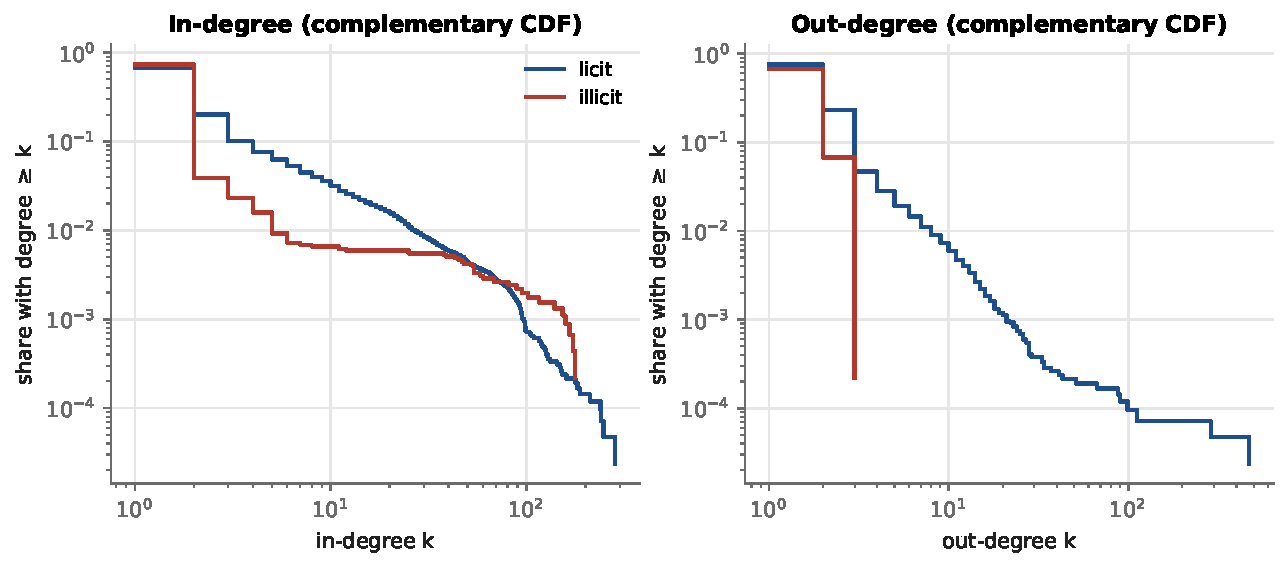
\includegraphics[width=\columnwidth]{../reports/figures/eda_degree.pdf}
  \caption{Degree distributions (share of transactions with degree $\geq k$).
  Illicit transactions never have more than three outputs.}
  \label{fig:degree}
\end{figure}
